\documentclass{article}

\usepackage[utf8]{inputenc}
\usepackage{amsfonts}
\usepackage{amsthm}
\usepackage{todonotes}
\usepackage{cryptocode}
\usepackage{algorithm,algorithmic}

\newcommand{\adv}{{\sf Adv}}
\newcommand{\madv}{\mathsf{Adv}}

\theoremstyle{definition}
\newtheorem{definition}{Definition}[section]

\title{Encrypted SNI: Privacy and Security}
\author{No Name}
\date{\today}

\begin{document}

\maketitle

\section{Introduction}

In this note we try formalize the privacy goals of Encrypted SNI \cite{ietf-tls-esni-04}.

\section{Goals}

\todo[inline]{writeme}

\section{Notation}

TLS is an authenticated key exchange protocol composed of sub-protocols. Importantly, TLS has
a handshake and record protocol. The handshake protocol uses handshake messages to perform
key exchange and its many facets, including, among other things, cryptographic algorithm
selection and peer authentication. Let $h \in \{0,1\}^{2^{16}}$ be a handshake message 
composed of arbitrary data, and let $\mathbf{H}$ be the set of possible handshake messages.

The record protocol uses messages with headers consisting 
of type, length, and version to send data between peers. This data is either a plaintext 
handshake message or encrypted blob. For our analysis, let $r = (d, p)$ be a 
record composed of direction $d \in \{0,1\}$ and payload $p \in \{0,1\}^{2^{16}}$. Let
$\mathbf{R}$ be the set of all possible records. Let $\mathbf{P} = \{0,1\}^{2^{16}}$ 
be the set of possible payloads. Note, by definition $\mathbf{H} \subset \mathbf{P}$.
Let $\mathsf{Message}$ be a function that returns the plaintext message for a given
record $r$, or nothing if the record is encrypted.

We model a TLS handshake as a trace of records and their metadata sent between a client and server. 
(Metadata may include, among other things, record lengths as observed on the wire.) 
Formally, let $\vec{t} = <r_0, r_1, \dots, r_n>$ be a trace of $n$ records, where 
$r_i = (d_i, p_i) \in \mathbf{R}$. Let $\mathbf{T}$ be a set of traces. 

Without loss of generality, in TLS 1.3, there are three types of messages observed
on the wire: ClientHello (CH), ServerHello (SH), and ApplicationData (AD). Let $\mathbf{CH}$ 
and $\mathbf{SH}$ be the set of possible CH and SH handshake messages generated by 
clients and servers, respectively. Each CH, SH, and AD message belongs to $\mathbf{P}$.

Let $N \in \{0,1\}^{2^{16} - 1}$ be a name, and let $\mathbf{N}$ be the set of names. 
CH messages typically carry names as one of their parameters.

Let $\mathsf{ClientConfig}$ be a set of parameters that determine a client's configuration,
including supported ciphersuites, named groups, extensions, etc. 
Let $\mathbf{CC}$ be the set of all client configuration parameters.
Similarly, let $\mathsf{ServerConfig}$ be a set of parameters that determine a server's configuration,
and let $\mathbf{SC}$ be the set of all client configuration parameters.
Clients produce CH messages to a given server, identified by its name $N$, and configuration
$\mathsf{ClientConfig}$, using a function $\mathsf{GenerateCH}: \mathbf{N} \times \mathbf{CC}$.
Servers produce SH messages (and do other parameter selection) based on a CH message and 
server configuration, using a function $\mathsf{GenerateSH}: \mathbf{CH} \times \mathbf{SC}$.

The function $\mathsf{Metadata}$ takes as input a CH or SH and returns the set of metadata,
or parameters, associated with the message, including the server name $N$, ciphersuite list,
named groups, and other extensions that are visible on the wire. The function
$\mathsf{PublicMetadata}$ returns the same output as $\mathsf{Metadata}$, except that
the server name is omitted. 

Using the notation above, every handshake is a probabilistic function of some server name $N$,
$\mathsf{ClientConfig}$, and $\mathsf{ServerConfig}$. In particular:
%
\begin{itemize}
    \item A client generates a CH message using $N$ and $\mathsf{ClientConfig}$.
    \item The recipient server generates a SH message using the input CH and $\mathsf{ServerConfig}$.
    \item The remainder of the handshake contains encrypted AD messages.
\end{itemize}
%
Thus, let $\mathsf{Handshake}$ be a function that takes as input $N$,
$cc = \mathsf{ClientConfig}$, and $sc = \mathsf{ServerConfig}$ and produces a trace 
$t = r_1, r_2, r_3, \dots$, where $\mathsf{Message}(r_1)$ is a CH and 
$\mathsf{Message}(r_2)$ is a SH. Let $\mathsf{PublicHandshake}$ be a similar
function that computes $t = r_1, r_2, r_3, \dots = \mathsf{Handshake}(t, cc, sc)$ and returns 
$t^v = \mathsf{PublicMetadata}(r_1), \mathsf{PublicMetadata}(r_2), r_3, \dots$. That is,
it returns publicly visible metadata associated from a handshake trace. 

Finally, we define a function $\mathsf{SNI}$ which takes as input a handshake trace $t$
and returns the name $N$ which was used to generate $t$. 

\section{Adversarial Model}

In this section, we describe two variants of an ESNI adversary: passive and active. We derive 
definitions from the classic ``find-and-choose'' notion of indistinguishability. Informally, 
in each game, the adversary \adv\ is given information about a game and must present two options
for the challenger. The challenger chooses one option at random and presents the result of some 
operation applied to the selected option to \adv, who must then identify which of 
the two options was selected. (This is typically the encryption of one message.) If the 
\adv's advantage in making this selection is negligibly later than $0.5$, then the options 
are indistinguishable under the challenger's operation.

In porting this definition to ESNI, we seek to capture indistinguishability of handshake traces
derived from names. That is, the challenger's operation is to generate a public handshake trace 
based on a randomly chosen name. Specifically, \adv\ chooses two names $N_0$ and $N_1$ during
a ``find'' phase, and presents them to the challenger $C$. $C$ then generates 
$t_b^v = \mathsf{PublicHandshake}(N_b)$, where $b \gets \{0,1\}$, and presents this to \adv. 
The adversary then presents its selection $b'$ to the challenger. The output of the game
depends on whether or not $b = b'$. This is shown in Figure \ref{fig:passive-game}.

\begin{figure}
    \centering
    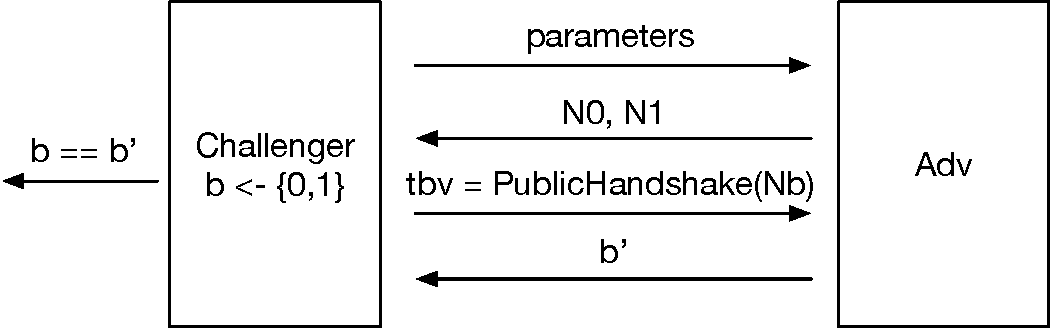
\includegraphics[scale=0.7]{esni_game.pdf}
    \caption{Passive ESNI Privacy game}
    \label{fig:passive-game}
\end{figure}

We capture this definition in the following {\sf NameGame}, which is defined in Algorithm \ref{alg:esnigame}.

\begin{algorithm}
\caption{{\sf NameGame}} 
\label{alg:esnigame}
\begin{algorithmic}[1]
  \STATE On input security parameter $\lambda$, $\mathbf{N}$, $\mathbf{CC}$, $\mathbf{SC}$, 
  and adversary \adv\, a challenger $C$ initializes \adv\ with $\mathbf{CC}$, $\mathbf{SC}$, and $\mathsf{N}$. 
  \STATE \adv\ presents the challenger with two distinct names $N_0$ and $N_1$, where $N_0 \not= N_1$.
  \STATE $C$ chooses a random bit $b$ and returns $t_b^v = \mathsf{PublicHandshake}(N_b)$ to \adv.
  \STATE \adv\ replies with a bit $b'$.
  \STATE Output $1$ if $b = b'$, otherwise output $0$.
\end{algorithmic}
\end{algorithm}

We say that \adv\ wins $\mathsf{NameGame}$ if it outputs $1$, i.e., if \adv\ was able to determine which
name the challenger used to produce the challenge handshake trace. We define the advantage \adv\ has in this 
game as $|\Pr[\mathsf{NameGame}(\lambda, \mathbf{N}, \mathbf{CC}, \mathbf{SC}, \madv)] - \frac{1}{2}|$. 

We say that a handshake trace is \emph{SNI agnostic} if, for all PPT adversaries \adv, \adv's advantage in 
winning $\mathsf{NameGame}$ is negligibly small in $\lambda$. 

\subsection{Active Adversary}

An active adversary has the ability to generate handshake traces at will. We assume servers are neither malicious nor compromised. 
Therefore, adapting our model for privacy requires extending $\mathsf{NameGame}$ to give \adv\ an oracle for producing handshake
traces with an SNI of its choosing. We define this oracle as $\mathcal{O}_H$, and it takes as input an SNI $N \in \mathbf{N}$
and returns a handshake trace $H(N) \in \mathbf{H}$. The modified game, called $\mathsf{ActiveNameGame}$, proceeds as follows:

\begin{algorithm}
\caption{{\sf ActiveNameGame}} 
\label{alg:active-esnigame}
\begin{algorithmic}[1]
  \STATE On input security parameter $\lambda$, $\mathbf{N}$, $\mathbf{CC}$, $\mathbf{SC}$, 
  and adversary \adv\, a challenger $C$ initializes \adv\ with $\mathbf{CC}$, $\mathbf{SC}$, 
  $\mathsf{N}$, and access to $\mathcal{O}_H$.
  \STATE \adv\ queries $\mathcal{O}_H$ with names values of its choosing from $\mathbf{N}$ at most $\mathsf{poly}(\lambda)$ times.
  \STATE \adv\ presents the challenger with two distinct names $N_0$ and $N_1$, where $N_0 \not= N_1$.
  \STATE $C$ chooses a random bit $b$ and returns $t_b^v = \mathsf{PublicHandshake}(N_b)$ to \adv.
  \STATE \adv\ continues querying $\mathcal{O}_H$ at most $\mathsf{poly}(\lambda)$ times.
  \STATE \adv\ replies with a bit $b'$.
  \STATE Output $1$ if $b = b'$, otherwise output $0$.
\end{algorithmic}
\end{algorithm}

As before, we say that \adv\ wins $\mathsf{ActiveESNIGame}$ if it outputs $1$. 
We define the advantage \adv\ has in this game as
$|\Pr[\mathsf{ActiveESNIGame}(\lambda, \mathbf{N}, \mathsf{config}, \madv)] - \frac{1}{2}|$. 
And we say that a handshake trace is \emph{SNI agnostic} with respect to an active attacker 
if \adv's advantage in winning $\mathsf{ActiveESNIGame}$ is negligibly small in $\lambda$.

Informally, \adv's advantage in these games depend on information leakage in handshake traces. 
Taken to an extreme, if all ClientHello, ServerHello, and encrypted handshake traces were 
identical, i.e., statistically indistinguishable among the set of possible messages that comprise
a trace, for any SNI, then no (message size) leakage exists.\footnote{We do not consider time-based
side channels that may compromise ESNI privacy.} Thus, we aim to show that, if these message
distributions are identical, then a given handshake trace is SNI-agnostic. This requires some
definition of \emph{uniformity} for a given message distribution. Recall the definitions of 
$\mathsf{GenerateCH}$ and $\mathsf{GenerateSH}$. The former takes as input a name and client
configuration, and produces a CH $m \in \mathbf{CH}$. We say $\mathsf{GenerateCH}$ is uniform
if for all $CH_i, CH_j \gets \mathsf{GenerateCH}(N, cc)$ for XXX

\section{ESNI Security}

Beyond handshake trace indistinguishability, ESNI security and privacy requires basic assumptions
about the secrecy of its encrypted contents. In particular, the contents of the ESNI extension must
be full bound to the handshake. We capture this in two ways: forward and backward bindings, defined 
below.

\begin{definition}
ESNI contents are \emph{forward-bound} to a handshake if it is not possible to decrypt handshake messages 
without both the handshake shared secret and ESNI shared secret.
\end{definition}

Forward binding restricts access to the traffic handshake secrets to the endpoints that possess both
the ESNI shared secret and handshake Diffie Hellman shared secret. This property is necessary for 
ESNI security. To illustrate this, consider the contrapositive towards a contradiction, wherein ESNI 
security is guaranteed in the absence of forward binding. An attack that violates this contradiction works 
as follows: A client generates a ClientHello with an ESNI payload and sends it to a server, which replies 
with a HelloRertryRequest in response. An on-path \adv\ intercepts the retry request and replies using
the client's original ESNI value and its own key share. The server then mistakenly uses the ESNI
value from the original ClientHello yet the key share from \adv, completing the handshake. In the
process, \adv\ learns the server certificate, which reveals the ESNI contents.

ESNI security also requires binding the encrypted contents to the ClientHello. We capture this 
notion of backward binding below.

\begin{definition}
ESNI contents are \emph{backward-bound} to a ClientHello if it is not possible to modify a ClientHello in 
any way without causing an ESNI check to fail.
\end{definition}

Backward binding restricts an adversary's abilities to passive eavesdropping and active packet generation.
To illustrate why this is necessary for ESNI security, consider, towards a contradiction, the contrapositive,
which states that ESNI security is possible if there is no backward binding. Consider the following attack
which violates this assumption. A client generates a ClientHello with an ESNI payload and sends it to a server.
An on-path \adv\ intercepts the message and replaces the key share with one of its own choosing. The server
completes the handshake and, similar to the attack above, reveals its certificate to \adv. 

Even if the key share were bound to the ClientHello, subtle attacks are also possible. In particular, consider
the following attack which relies on tickets and resumption state. \adv\ connects to a target server, using ESNI 
with a guess name {\tt example.com}, and receives a ticket upon successful negotiation. A client then
generates a ClientHello with an ESNI payload and no resumption PSK binder. \adv\ then attaches its ticket and 
PSK binder to the ClientHello and forwards the result to the server. If the server checks that the name in 
the ticket matches that of the ESNI payload and behaves differently as a result, e.g., by completing the handshake
without resumption or by aborting the connection, \adv\ learns information about the ESNI. This allows \adv\ to
conduct a dictionary-like attack on victim ESNIs.

\begin{theorem}
If ESNI is secure (as per one of the definitions above), then ESNI contents are \emph{backward-bound} and \emph{forward-bound}.
\end{theorem}

%%% XXX(caw): prove this by counter example?

\begin{theorem}
If ESNI is secure (as per one of the definitions above), then handshake traces are SNI-agnostic.
\end{theorem}

%%% XXX(caw): prove by building a distinguisher?


%%% goal: if forward and backward bound, and if SNI-agnostic, then ESNI is secure.
% contradiction: if forward and backward bound and SNI-agnostic, then not ESNI secure
% approach: 
% - backward bound: adv can only generate CH messages // Query to Bind for GenerateCH output goes away since adv cannot modify victim (CHs+State)
%    (Bind can be called with name CH that adv produces itself)
%    (adv presents CH+{state}) to challenger)
% - forward bound: adv cannot obtain name from handshake it did not generate // Query to Reveal on traces produced by GenerateCH goes away
% - SNI-agnostic: adv is left with ability to forward CHs from GenerateCH and create its own and bind them

% game hopping sequence:
% game 0: the modified game above 
% game 1: replace challenger trace with trace from random name // follows from IND of traces
% --> adv outputs the *same* in both cases, so therefore the trace leaks nothing, and adv probability is no better than 1/2 + Pr[distinguish traces]

%% Q: show that forward/backward bind in the game above, without them, lead to some attack. 
% forward: adv can use its reveal query on trace to learn ESNI.
% backward: maybe not part of the game?

\bibliographystyle{plain}
\bibliography{references}

\end{document}
